\documentclass[a4paper]{book}

\usepackage{geometry}
% make full use of A4 papers
\geometry{margin=1.5cm, vmargin={0pt,1cm}}
\setlength{\topmargin}{-1cm}
\setlength{\paperheight}{29.7cm}
\setlength{\textheight}{25.1cm}

% auto adjust the marginals
\usepackage{marginfix}

\usepackage{amsfonts}
\usepackage{amsmath}
\usepackage{amssymb}
\usepackage{amsthm}
%\usepackage{CJKutf8}   % for Chinese characters
\usepackage{ctex}
\usepackage{enumerate}
\usepackage{graphicx}  % for figures
\usepackage{layout}
\usepackage{multicol}  % multiple columns to reduce number of pages
\usepackage{mathrsfs}  
\usepackage{fancyhdr}
\usepackage{subfigure}
\usepackage{tcolorbox}
\usepackage{tikz-cd}
\usepackage{listings}
\usepackage{xcolor} %代码高亮
\usepackage{braket}
%------------------
% common commands %
%------------------
% differentiation
\newcommand{\gen}[1]{\left\langle #1 \right\rangle}
\newcommand{\dif}{\mathrm{d}}
\newcommand{\difPx}[1]{\frac{\partial #1}{\partial x}}
\newcommand{\difPy}[1]{\frac{\partial #1}{\partial y}}
\newcommand{\Dim}{\mathrm{D}}
\newcommand{\avg}[1]{\left\langle #1 \right\rangle}
\newcommand{\sgn}{\mathrm{sgn}}
\newcommand{\Span}{\mathrm{span}}
\newcommand{\dom}{\mathrm{dom}}
\newcommand{\Arity}{\mathrm{arity}}
\newcommand{\Int}{\mathrm{Int}}
\newcommand{\Ext}{\mathrm{Ext}}
\newcommand{\Cl}{\mathrm{Cl}}
\newcommand{\Fr}{\mathrm{Fr}}
% group is generated by
\newcommand{\grb}[1]{\left\langle #1 \right\rangle}
% rank
\newcommand{\rank}{\mathrm{rank}}
\newcommand{\Iden}{\mathrm{Id}}

% this environment is for solutions of examples and exercises
\newenvironment{solution}%
{\noindent\textbf{Solution.}}%
{\qedhere}
% the following command is for disabling environments
%  so that their contents do not show up in the pdf.
\makeatletter
\newcommand{\voidenvironment}[1]{%
  \expandafter\providecommand\csname env@#1@save@env\endcsname{}%
  \expandafter\providecommand\csname env@#1@process\endcsname{}%
  \@ifundefined{#1}{}{\RenewEnviron{#1}{}}%
}
\makeatother

%---------------------------------------------
% commands specifically for complex analysis %
%---------------------------------------------
% complex conjugate
\newcommand{\ccg}[1]{\overline{#1}}
% the imaginary unit
\newcommand{\ii}{\mathbf{i}}
%\newcommand{\ii}{\boldsymbol{i}}
% the real part
\newcommand{\Rez}{\mathrm{Re}\,}
% the imaginary part
\newcommand{\Imz}{\mathrm{Im}\,}
% punctured complex plane
\newcommand{\pcp}{\mathbb{C}^{\bullet}}
% the principle branch of the logarithm
\newcommand{\Log}{\mathrm{Log}}
% the principle value of a nonzero complex number
\newcommand{\Arg}{\mathrm{Arg}}
\newcommand{\Null}{\mathrm{null}}
\newcommand{\Range}{\mathrm{range}}
\newcommand{\Ker}{\mathrm{ker}}
\newcommand{\Iso}{\mathrm{Iso}}
\newcommand{\Aut}{\mathrm{Aut}}
\newcommand{\ord}{\mathrm{ord}}
\newcommand{\Res}{\mathrm{Res}}
%\newcommand{\GL2R}{\mathrm{GL}(2,\mathbb{R})}
\newcommand{\GL}{\mathrm{GL}}
\newcommand{\SL}{\mathrm{SL}}
\newcommand{\Dist}[2]{\left|{#1}-{#2}\right|}

\newcommand\tbbint{{-\mkern -16mu\int}}
\newcommand\tbint{{\mathchar '26\mkern -14mu\int}}
\newcommand\dbbint{{-\mkern -19mu\int}}
\newcommand\dbint{{\mathchar '26\mkern -18mu\int}}
\newcommand\bint{
	{\mathchoice{\dbint}{\tbint}{\tbint}{\tbint}}
}
\newcommand\bbint{
	{\mathchoice{\dbbint}{\tbbint}{\tbbint}{\tbbint}}
}





%----------------------------------------
% theorem and theorem-like environments %
%----------------------------------------
\numberwithin{equation}{chapter}
\theoremstyle{definition}

\newtheorem{thm}{Theorem}[chapter]
\newtheorem{axm}[thm]{Axiom}
\newtheorem{alg}[thm]{Algorithm}
\newtheorem{asm}[thm]{Assumption}
\newtheorem{defn}[thm]{Definition}
\newtheorem{prop}[thm]{Proposition}
\newtheorem{rul}[thm]{Rule}
\newtheorem{coro}[thm]{Corollary}
\newtheorem{lem}[thm]{Lemma}
\newtheorem{exm}{Example}[chapter]
\newtheorem{rem}{Remark}[chapter]
\newtheorem{exc}[exm]{Exercise}
\newtheorem{frm}[thm]{Formula}
\newtheorem{ntn}{Notation}

% for complying with the convention in the textbook
\newtheorem{rmk}[thm]{Remark}


%\lstset{
%	backgroundcolor=\color{red!50!green!50!blue!50},%代码块背景色为浅灰色
%	rulesepcolor= \color{gray}, %代码块边框颜色
%	breaklines=true,  %代码过长则换行
%	numbers=left, %行号在左侧显示
%	numberstyle= \small,%行号字体
%	keywordstyle= \color{blue},%关键字颜色
%	commentstyle=\color{gray}, %注释颜色
%	frame=shadowbox%用方框框住代码块
%}
\lstset{
	columns=fixed,       
	numbers=left,                                        % 在左侧显示行号
	numberstyle=\tiny\color{gray},                       % 设定行号格式
	frame=none,                                          % 不显示背景边框
	backgroundcolor=\color[RGB]{245,245,244},            % 设定背景颜色
	keywordstyle=\color[RGB]{40,40,255},                 % 设定关键字颜色
	numberstyle=\footnotesize\color{darkgray},           
	commentstyle=\it\color[RGB]{0,96,96},                % 设置代码注释的格式
	stringstyle=\rmfamily\slshape\color[RGB]{128,0,0},   % 设置字符串格式
	showstringspaces=false,                              % 不显示字符串中的空格
	language=c++,                                        % 设置语言
}

%----------------------
% the end of preamble %
%----------------------

\begin{document}
\pagestyle{empty}
\pagenumbering{roman}

%\tableofcontents
%\clearpage

%\pagestyle{fancy}
%\fancyhead{}
%\lhead{Qinghai Zhang}
%\chead{Notes on Algebraic Topology}
%\rhead{Fall 2018}


\setcounter{chapter}{0}
\pagenumbering{arabic}
% \setcounter{page}{0}

% --------------------------------------------------------
% uncomment the following to remove these environments 
%  to generate handouts for students.
% --------------------------------------------------------
% \begingroup
% \voidenvironment{rem}%
% \voidenvironment{proof}%
% \voidenvironment{solution}%


% each chapter is factored into a separate file.

\chapter{微分方程数值解第一次作业解答}
%\begin{lstlisting}
%int main(){
%  double d;
%  int i;
%  return i;
%}
%\end{lstlisting}
% The main ingredients of snacks are sugar and fat;
%  the main ingredients of math are logic and set theory.

文档当make anwser math design后都会生成在tex/目录中,make run可执行文件在exc2/src中,make test测试可执行文件在exc2/test,输入文件在input/中.

\section{第一题}
已知二重网格求解的方程为
\begin{equation}
	TG
	\begin{bmatrix}
	 \mathbf{w}_k \\ 
	 \mathbf{w}_{k^{'}}
	 \end{bmatrix} 
	=
	\begin{bmatrix}
	\lambda^{\nu_1 + \nu_2}_k s_k & \lambda^{\nu_1}_k \lambda^{\nu_2}_{k^{'}} s_k \\
	\lambda^{\nu_1}_{k^{'}} \lambda^{\nu_2}_{k} c_k  & \lambda^{\nu_1 + \nu_2}_{k^{'}} c_k
	\end{bmatrix} 
	\begin{bmatrix}
	\mathbf{w}_k \\ 
	\mathbf{w}_{k^{'}}
	\end{bmatrix}
	=:
	\begin{bmatrix}
	c1 & c2 \\
	c3 & c4
	\end{bmatrix}
	\begin{bmatrix}
	\mathbf{w}_k \\ 
	\mathbf{w}_{k^{'}}
	\end{bmatrix}  \qquad  1 \leq k \leq n/2
\end{equation}
其中$k^{'} = n - k$因为使用的是加权Jacobi松弛,所以$\lambda_k = 1 - 2w\sin(\frac{k \pi}{2n})$.结合$s_k = \sin^2(\frac{\pi k}{2n}), c_k = \cos^2(\frac{\pi k}{2n})$.可画出damping coefficient $c1,c2,c3,c4$与$k$之间的如下图像1.1(exc1/ 中的matlab程序运行即可画出此图).

\begin{figure}
	\centering
	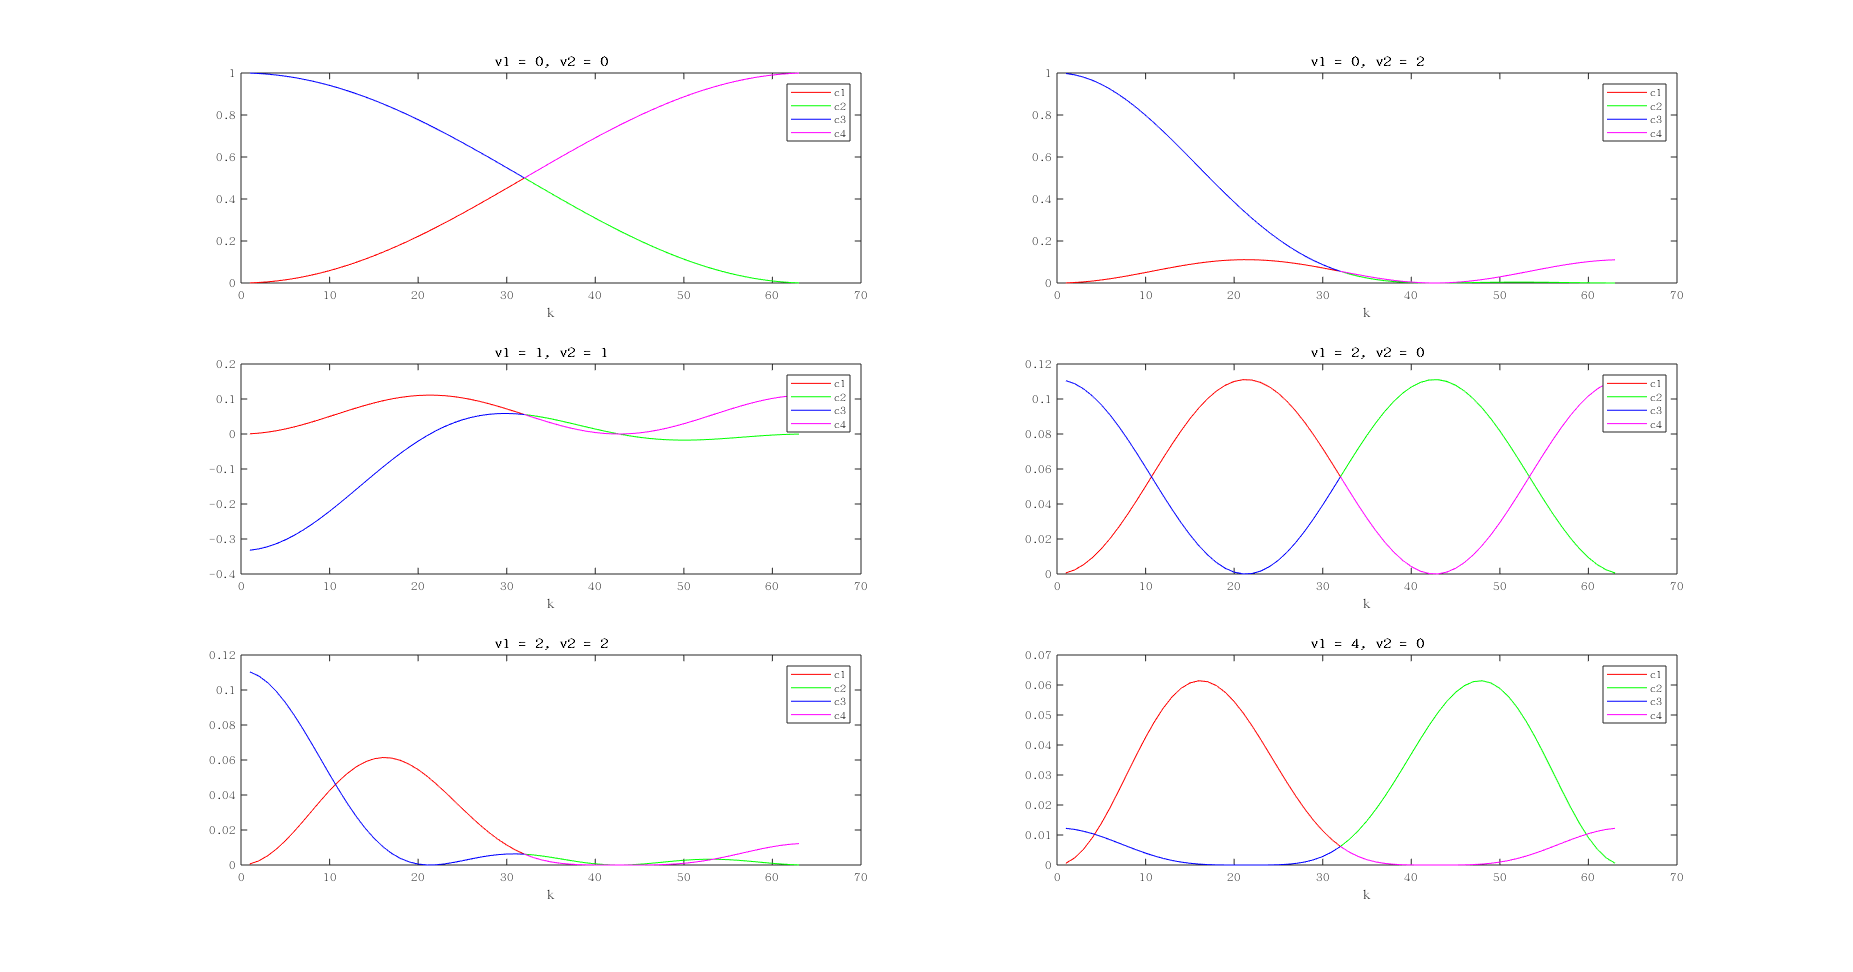
\includegraphics[width=15cm,height=20cm]{../exc1/exc1.png}
	\caption{damping coefficient 在不同$\nu$的条件下关于$k$的函数图像}
\end{figure}

\section{第二题}
exc2中为程序,src/中是源码,test/包含测试程序,input/包含输入文件.若要自定义输入文件,需要参考input/allinput.txt和其包含的文件的示范文件exampleinput.txt.目前没有增加忽略注释功能需要去除所有注释.

\section{第三题}
根目录make run会运行$u(x) = \exp(\sin(x))$当$n = 128,256,512,1024$的V-cycle迭代结果,每步都输出$e,r$的无穷范数和收敛速率.

\section{第四题}
不能收敛到$2.2 \times 10^{-22}$, make run4 将会输入input/allinput4.txt将停止条件设为$2.2 \times 10^{-22}$,迭代50次或更多都不能达到停止条件.

\section{第五题}
使用$u(x) = \sin(x)$,是一个边界为0的边界条件,并且在make run和make run4中已经同时进行运算输出了.


\end{document}


%%% Local Variables: 
%%% mode: latex
%%% TeX-master: t
%%% End: 

% LocalWords:  FPN underflows denormalized FPNs matlab eps IEEE iff
% LocalWords:  cardinality significand quadratically bijection unary
%  LocalWords:  contractive bijective postcondition invertible arity
%  LocalWords:  subspaces surjective injective monomials additivity
%  LocalWords:  nullary Abelian abelian finitary eigenvectors adjoint
%  LocalWords:  eigenvector nullspace Hermitian unitarily multiset
%  LocalWords:  nonsingular nonconstant homomorphism homomorphisms
%  LocalWords:  isomorphically indeterminates subfield isomorphism
%  LocalWords:  nondefective diagonalizable contrapositive cofactor
%  LocalWords:  submatrix nilpotent positivity orthonormal extremum
%  LocalWords:  Jacobian nonsquare semidefinite nonnegative RHS LLS
%  LocalWords:  roundoff closedness
